\chapter{Experimental Setup}

\section{RHIC}
The Relativistic Heavy Ion Collider (RHIC) is a superconducting charged hadron collider located at Brookhaven Nation Labs (BNL) in Upton, NY. RHIC is capable of accelerating heavy ions such as Au (gold) or Cu (copper) nuclei to energies of 200 GeV per nucleon. RHIC is also capable of accelerating lighter ions such as protons, deuteron, and helium to 200 GeV per nucleon and 510 GeV per nucleon in the case of protons. There are currently 2 major detector experiments operating in interaction regions around the RHIC ring: PHENIX and STAR. RHIC typically is operating for 5.5 months every year in what is called a "Run". 
A chain of smaller accelerators is used to "feed" the ions into RHIC, where they are accelerated (or decelerated in some circumstances) to the desired collision energy. For heavy ions such as Au, the process is listed below.  . When the ions exit the Tandem Van De Graaff, . Then the Booster Synchrotron to 95 MeV per nucleon
\begin{enumerate}
  \item{} A pulsed sputter Au ion source to generates negative ions in the Tandem Van De graaff.
  \item{} The ions are passed through an electron stripping foil to achieve a positive 12 charge and accelerated to 1 MeV per nucleon.
  \item{} The ions pass through magnets to further strip electrons and filter charge, yielding to a positive 32 charge state.
  \item{} The ions are sent to the Booster Synchrotron which accelerates them to 95 MeV per nucleon and leaves them at a positive 77 charge.
  \item{} The ions enter the Alternating Gradient Synchrotron (AGS) in 24-ion bunches. The ions are debunched and rebunched into 4 bunches and then accelerated to 10.8 GeV per nucleon.
  \item{}  The bunches then exit the AGS one at a time, where their Au ions are stripped of their 2 remaining electrons, yielding a final charge state of  positive 79. Finally, the bunches are transferred to their respective buckets in RHIC.
\end{enumerate}

There has been 16 "Runs" so far but the relevant run for this thesis was Run 15 taken in 2015 which was p+Au collisions at 200 GeV per nucleon.
\section{PHENIX }
\begin{figure}[!h]
\begin{center}
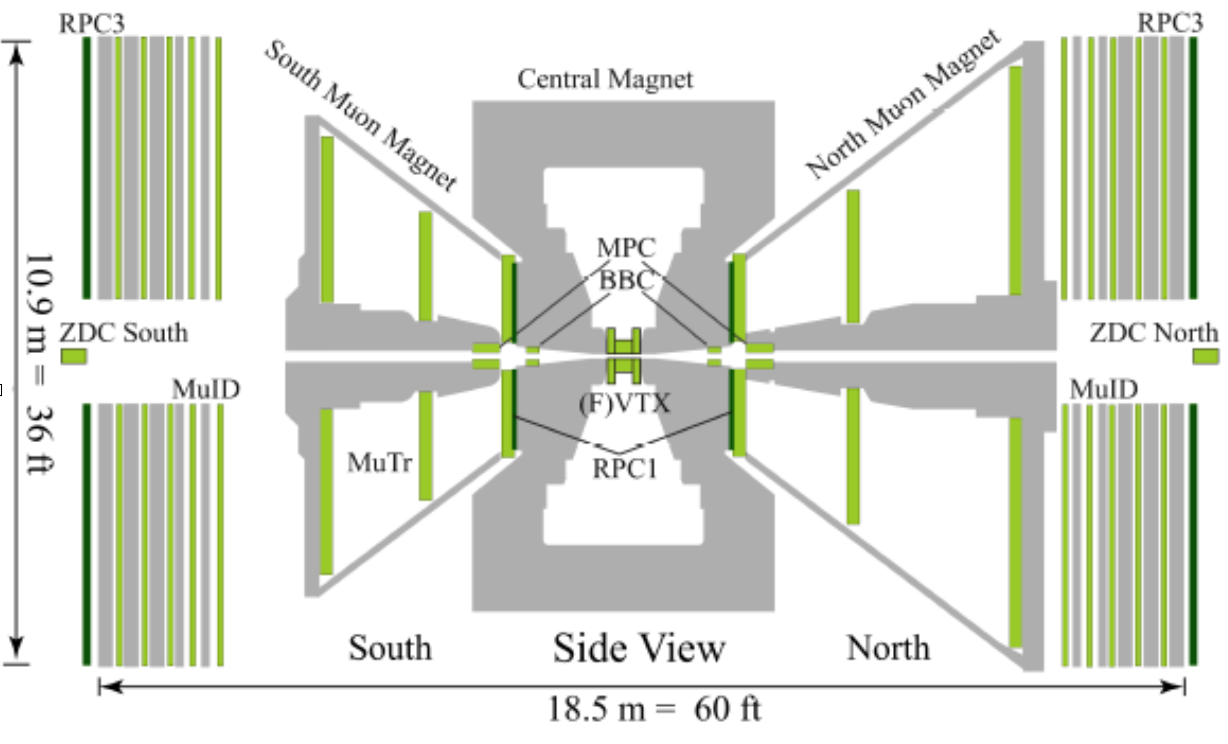
\includegraphics[width=0.5\linewidth]{figs/phenix_schematic.png}
\caption{TBA}
\end{center}
\end{figure}
\subsection{Event Categorization Detectors}
Talk about all detectors in this category including ZDC briefly.
\subsubsection{Beam Beam Counter (BBC)}
The Beam Beam Counter (BBC) is a multipurpose detector used to determine
the event start time, vertex, centrality, and is also one of several detectors capable
of measuring ?EP . The BBC is composed of two mirror image arrays, a South and
a North Arm, that surround the beam pipe 144 cm on opposite sides of the nominal
collision point just behind the Central Magnet, covering 3.0 < |$\eta$| < 3.9 and 2 $\pi$ radians in
azimuth. Each BBC arm is made of 64 elements each composed of a 3-cm length quartz
Cherenkov radiator connected to a 1-in diameter Hamamatsu R6178 mesh dynode
PMT (photomultiplier tube), as shown in Fig (TBA). The outer and inner diameters
of the BBC are 30 cm and 10 cm, respectively, allowing for a 1 cm clearance of the
beam pipe.
With a timing resolution of 52�4 ps, the BBC is used to mark the event start
time for the entire PHENIX detector by averaging the emitted particles arrival time
at each BBC arm. The timing difference between each arm is used to determine the
collision?s z-vertex or simply vertex or z by
\begin{equation}
z = c \frac{T_S ? T_N}{2},
\end{equation}

where TS,N are the particle's arrival times for each arm and c is the speed of light.
In 200-GeV Au+Au collisions the BBC vertex resolution is 0.5 cm and the (x,y)
collision position is always assumed to be (0,0). Determining the z-vertex aids in
particle track reconstruction and in eliminating events that occurred outside the
PHENIX acceptance of 30 cm $<$ z $<$ 30 cm.
The BBC is also used as a Level-1 minimum-bias (min-bias) trigger detector,
which initiates the recording of an event. Here, min-bias refers to applying the
minimum number of requirements to an event before acceptance. 
In Run 15, the requirement for a min-bias trigger is $>$ 0 PMTs above threshold. However in addition to providing the min-bias trigger for Run 15,
the BBC was used to implement a high-multiplicity trigger in order to enhance the amount of the top $5\%$ highest multiplicity events. 
The enhancement can be seen in Figure (TBA). This will be further discussed in Sec. (TBA).
Also, the BBC was used to determine the event centrality by summing the charge collection of each
BBC element; it is assumed the larger the charge collection the more central the
event. This will be further discussed in Sec. (TBA) Moreover, the BBC can measure
event plane using. For further BBC event plane calculation details see section (TBA).
\begin{figure}[!h]
\begin{center}
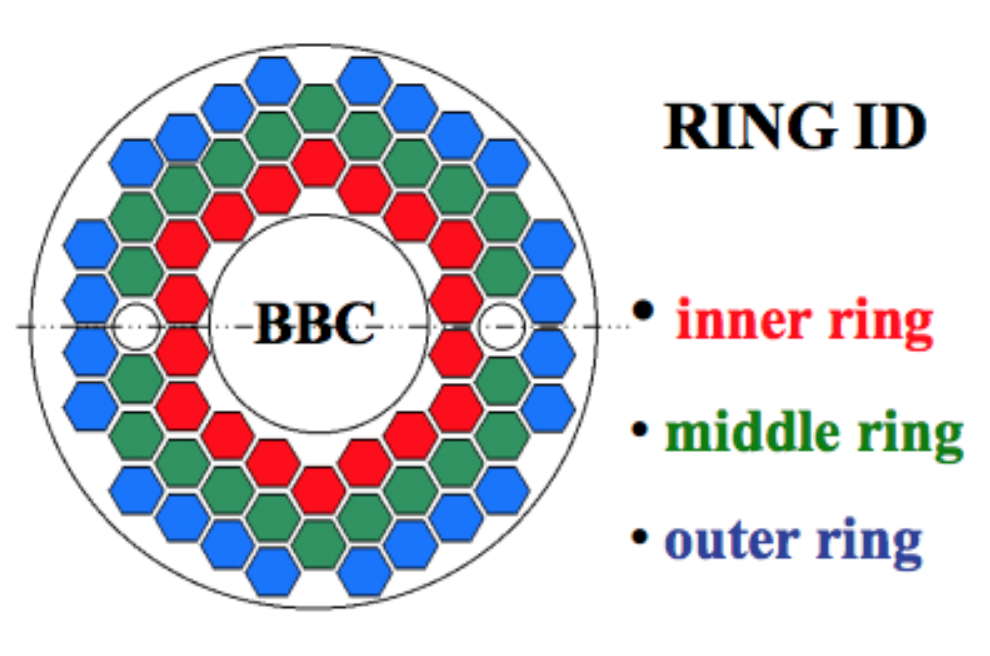
\includegraphics[width=0.4\linewidth]{figs/bbc_ring_schematic.png}
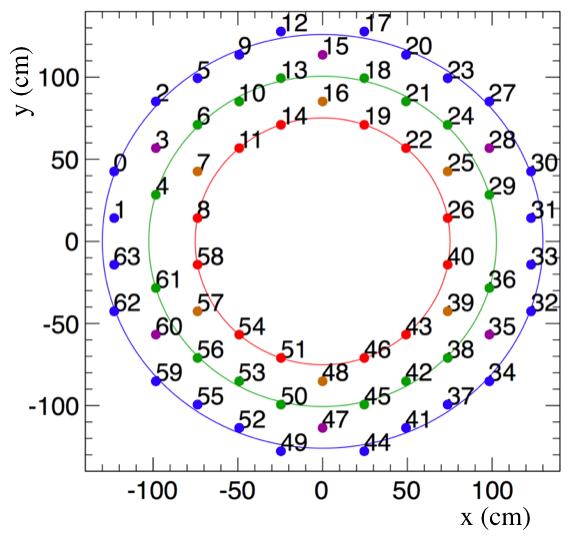
\includegraphics[width=0.4\linewidth]{figs/bbc_rings.png}
\caption{TBA}
\end{center}
\end{figure}
\subsection{Forward Rapidity Detectors}
\subsubsection{Forward Vertex Detector (FVTX)}
The Forward Silicon Vertex Tracker (FVTX) consists of two identical endcaps covering a psuedorapidity range of 1 $<|\eta|<$ 3 
and an azimuth range of $ 0 < \phi < 2\pi$.
Each one has four stations of silicon mini-strip sensors with a pitch of 75 $\mu m$ arranged in the radial direction around the beam pipe.
The basic unit of construction is a wedge that has a silicon strip sensor and read-out chips. There are 4 FVTX layers in each endcap and 
they vary in radial extent. 
\begin{figure}
\begin{center}
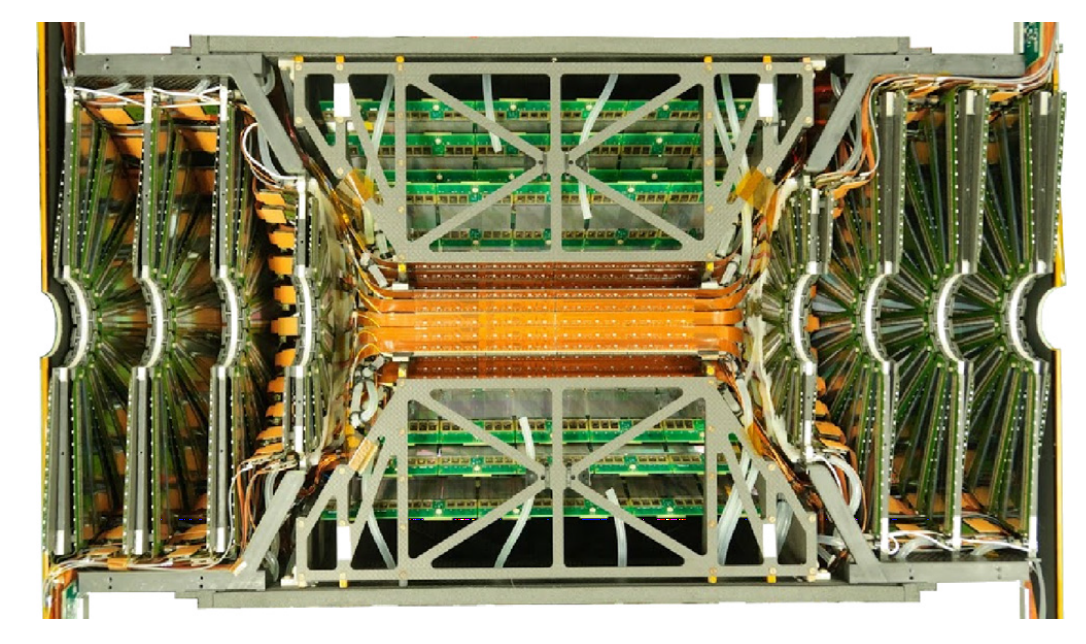
\includegraphics[width=0.4\linewidth]{figs/fvtx_cutaway.png}
\caption{FVTX/VTX cut}
\end{center}
\end{figure}
\subsubsection{FVTX Clustering}
\subsection{Midrapidity Detectors}
\subsubsection{Drift Chamber}
The Drift Chamber (DC) consists of two gas wire
chambers, one located in each arm, and is used to measure particle trajectories in the r $\phi$
plane with the primary goals of measuring the particles transverse momentum (pT) and
providing an anchoring point for the tracking.
The DC is the innermost subsystem in the central arms, 2 m from the z-axis, placing
them in a residual magnetic field of 0.6 kG. Each DC is cylindrical in design and covers 2
m along the beam direction and is 0.4 m thick, with the DC located in the West arm being
a mirror image of that located in the East arm. A gas mixture of $50\%$ Ar and $50\%$ Ethane
is used in each of the detectors.
Each detector is divided into 20 equal sectors covering 4.5 degrees in $\phi$. Each sector contains six
types of wire modules stacked radially and labeled X1, U1, V1, X2, U2, V2, respectively from
the inside out. The X wires run parallel to the beam to perform precise 4 $\phi$ measurements
while the U and V wires are set at small angles of about 6 degrees
relative to the X wires to provide
information about the z position of the track. A diagram of the wire layout in each sector
is shown in Figure (TBA). In total, the DC consists of 6500 anode wires leading to 13,000
readout channels, with a measured single wire resolution of 165 �m and a spatial resolution
of 2mm.
\subsubsection{Pad Chambers}
The Pad Chambers (PC) are multiwire proportional
chambers which consists of three separate layers of detectors measuring precise hit positions
and making up the bulk of the PHENIX tracking system. The innermost layer, PC1, is
located in both the East and West arms immediately outside the DC, providing a measurement
of the z position at the back plane of the DC. The second layer, PC2, is located
behind the RICH in the West arm only. The outer layer, PC3, is located just inside the
EMCal in both arms and provides a second point on the straight line trajectories of the
tracks through the detector, outside of the magnetic field.
\subsubsection{Ring Imaging Cherenkov Detector}
The Ring Imaging Cherenkov (RICH) detector is located immediately behind the PC1 and provides the primary 
electron identification for PHENIX, in conjunction with the EM Cal. The RICH consists of two identical
detectors located in each arm and provides e over pi discrimination below the pion Cherenkov threshold of
4.65 GeVc in the CO2 gas used in the detectors.
\subsubsection{EM Cal}
The Electromagnetic Calorimeter (EM Cal) is the outermost subsystem in the central arms and is designed primarily
to measure the energies and positions of photons and electrons. It also plays a key role in the identification of as well
as providing triggering for rare events. Two different EM Cal designs were utilized with 6 sectors based on a lead-
scintillator design and 2 sectors based on a lead-glass design. The two different designs were chosen
deliberately as each provides advantages and disadvantages, for instance the lead glass has a better energy resolution,
while the lead scintallator has better linearity and timing.
\subsubsection{Silicon Vertex Detector (SVX)}
\subsection{DAQ}
Both the event rate and the event size are large at RHIC and therefore a system which can make decisions event by event
and select events containing rare signals is necessary. The online data acquisition system (DAQ) and collects signals
from the various subsystems and then processes the event acceptance decision based on various triggers.
\subsubsection{Triggering}
\section{Event Reconstruction and Characterization}
\subsection{Central Arm Tracking}
\begin{figure}
\begin{center}
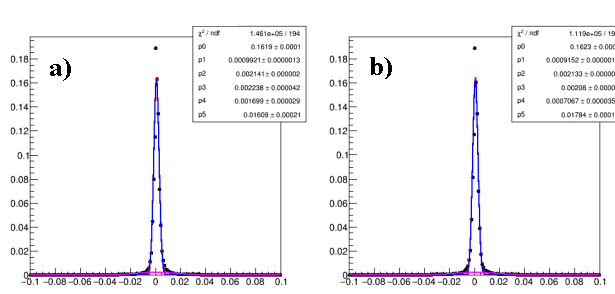
\includegraphics[scale=0.35]{figs/pc3dphi.png}
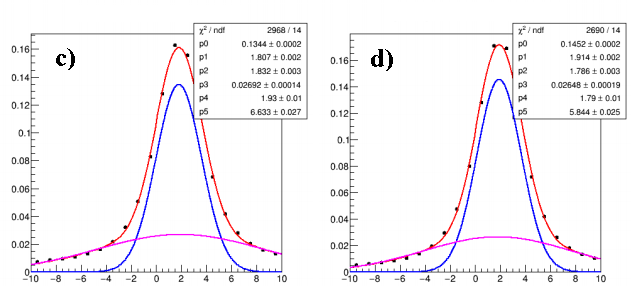
\includegraphics[scale=0.35]{figs/pc3dz.png}
\end{center}
\caption{TBA}
\end{figure}
\subsection{CNT Tracks Simulation}
\subsection{Centrality Determination}
\subsection{Vertex Determination}
\begin{figure}
\begin{center}
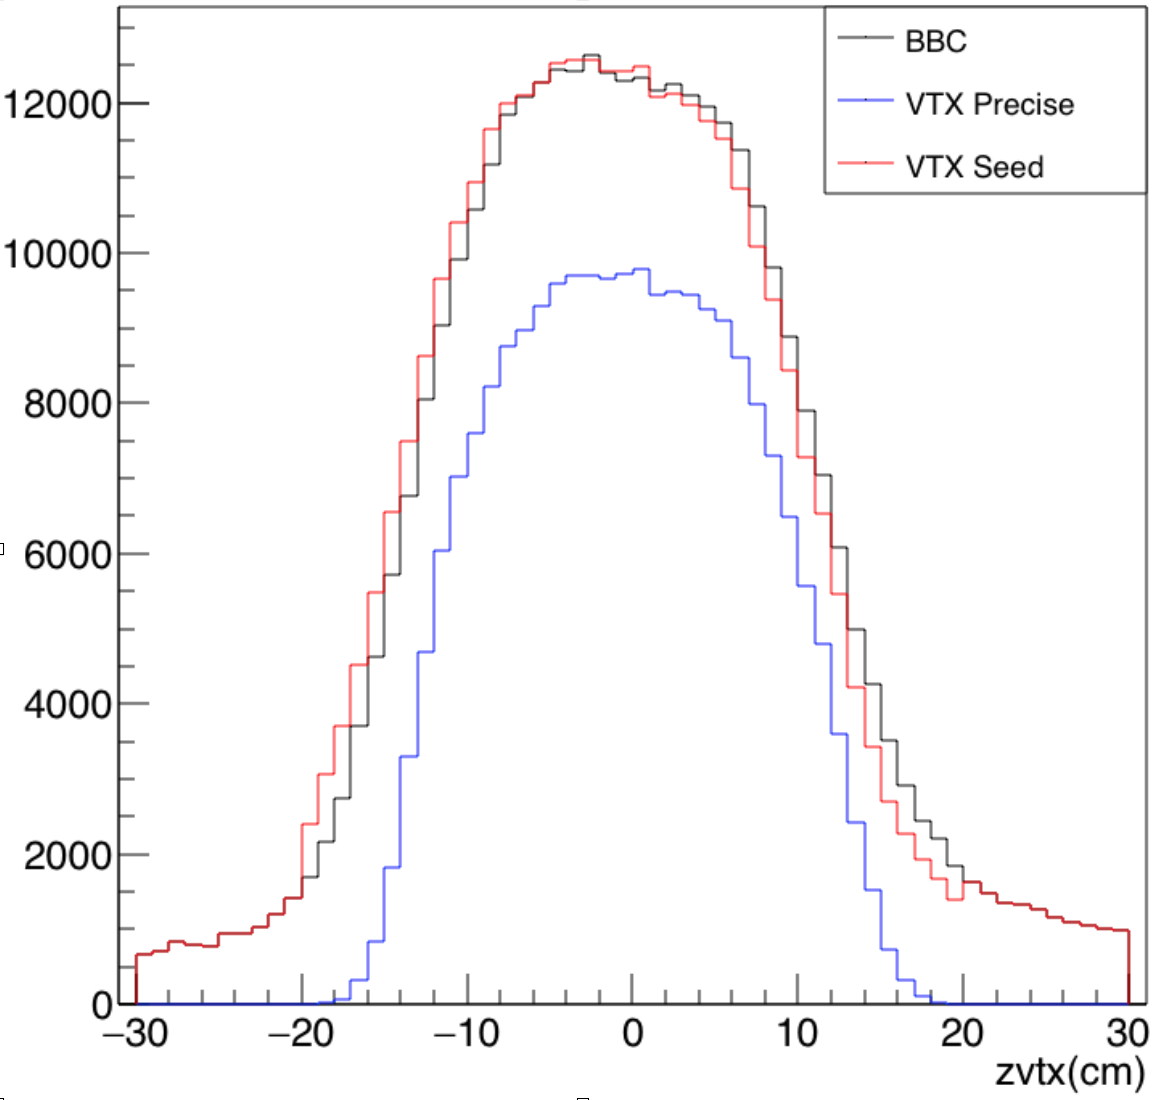
\includegraphics[scale=0.35]{figs/zvtx_distributions.png}
\end{center}
\caption{TBA}
\end{figure}
\section{Run15 pAu Dataset}
\begin{figure}
\begin{center}
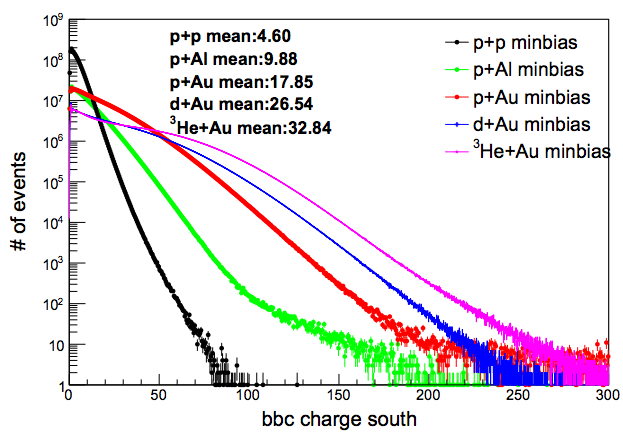
\includegraphics[scale=0.35]{figs/bbc_q_comp.png}
\end{center}
\caption{TBA}
\end{figure}
\subsection{Beam Geometry Effects}
\begin{figure}
\begin{center}
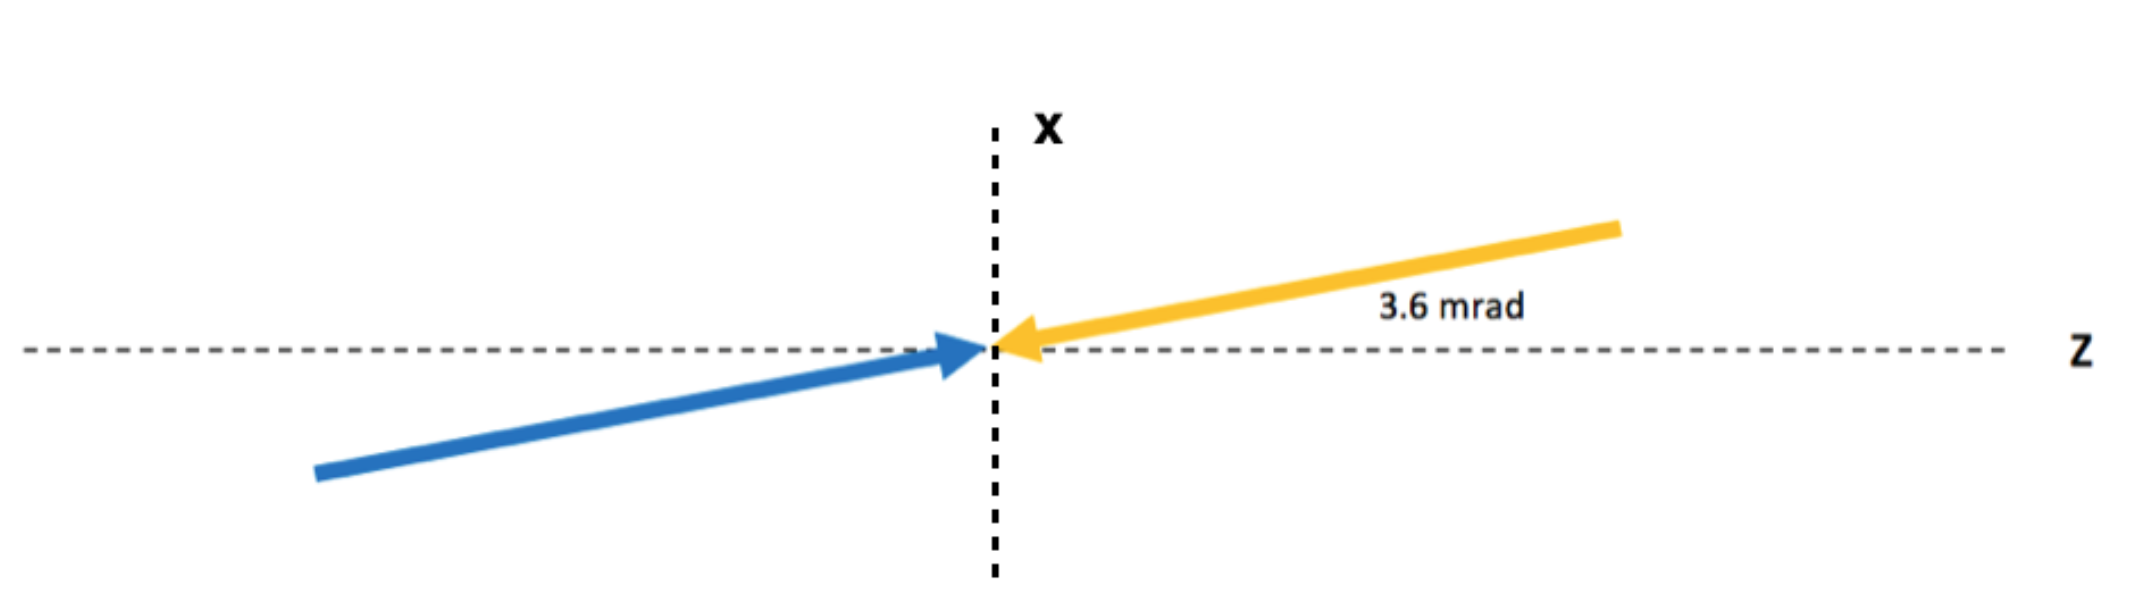
\includegraphics[width=0.65\linewidth]{figs/beam_angle.png}
\caption{A vector diagram illustrating the yellow and blue beam angle.}
\end{center}
\end{figure}


